\chapter{Research methodology and implementation}
In this chapter the author is designing the methodology to be followed in the experiments. This is an important step, as building it correctly will lead to significant and meaningful results.
We discuss three phases: data acquisition and preprocessing, price forecasting and predictor's importance.

In the first phase, all the necessary data will be downloaded with the finest possible granularity.
When studying broader timespans, it will be aggregated.

In the last two phases the author explains the design of the experiments: the same procedure will be used to analyze in an hourly, daily and monthly fashion, changing the parameters for every case.
On the other hand, for the yearly study, as there is not enough data to perform an statistical study, a descriptive and visual analysis will be performed.

\section{Data acquisition and preprocessing}


\section{Price forecasting}
The library used to perform forecasts is \textit{sktime}: it simplifies the implementation, reducing boilerplate code and making the scripts cleaner.

\subsection{Models to compare}
We will test different models, analyzing which of them work better. The following are ML-based:
\begin{itemize}
    \item k-Nearest Neighbors (kNN)
    \item Random Forest (RF)
    \item Gradient Boosted Trees (GBT)
    \item Support Vector Machine (SVM)
\end{itemize}
All of them are implemented in \textit{scikit-learn} and integrated in \textit{sktime} by the use of \textit{make\_reduction()} function. Some based on statistics are also used:
\begin{itemize}
    \item AutoARIMA
    \item AutoETS
\end{itemize}
The first is wrapped from \textit{pmdarima} package. A dummy regressor and Prophet performances are also studied, the dummy regressor score will act as baseline.

To compare the performance of different models the author will use the Mean Absolute Error (MAE) loss functionss described in Equation \ref{eq:mae}:

\begin{equation}
 \text{MAE}(y, \hat{y}) = \frac{ \sum_{i=0}^{N - 1} |y_i - \hat{y}_i| }{N}
 \label{eq:mae}
\end{equation}

Two well known strategies used to divide data for training and model evaluation are holdout and cross-validation.
In the former, data is partitioned in two splits, train and test, e.g. 80\% train and 20\% test.
The problem with this strategy is that we are only assessing the performance of the model in a reduced portion of data.
On the other hand, if we use cross-validation we divide the data in multiple folds: on an iterative process, one is reserved for testing and the rest for training, changing the test fold on every iteration.
At the end, we manage to assess the performance in the complete dataset.

\noindent But using k-fold cross validation is not suitable for time series forecasting \cite{cross-validation-types}:
\begin{enumerate}
    \item Test data can appear before train data.
    \item Data leakage can happen if test data appears after train folds, as the model knows extra information about the future.
\end{enumerate}

There exist other cross validation techniques that solve this problem, for example sliding or expanding windows.
In sliding windows splitters, the folds are created by scrolling a window of constant size through data.
This window is divided into train and test, maintaining the size of both partitions on all the windows.

In the case of expanding windows its size is not constant but it grows. Concretely, the test partition remains the same through different windows and the train one grows collecting all the previous observations.
In Figure \ref{fig:sliding-expanding-windows} the author exposes a comparison between both strategies.

\begin{figure}[H]
\centering
    \caption{Sliding vs expanding windows \cite{sliding-expanding-windows}.}
    \label{fig:sliding-expanding-windows}
    \fbox{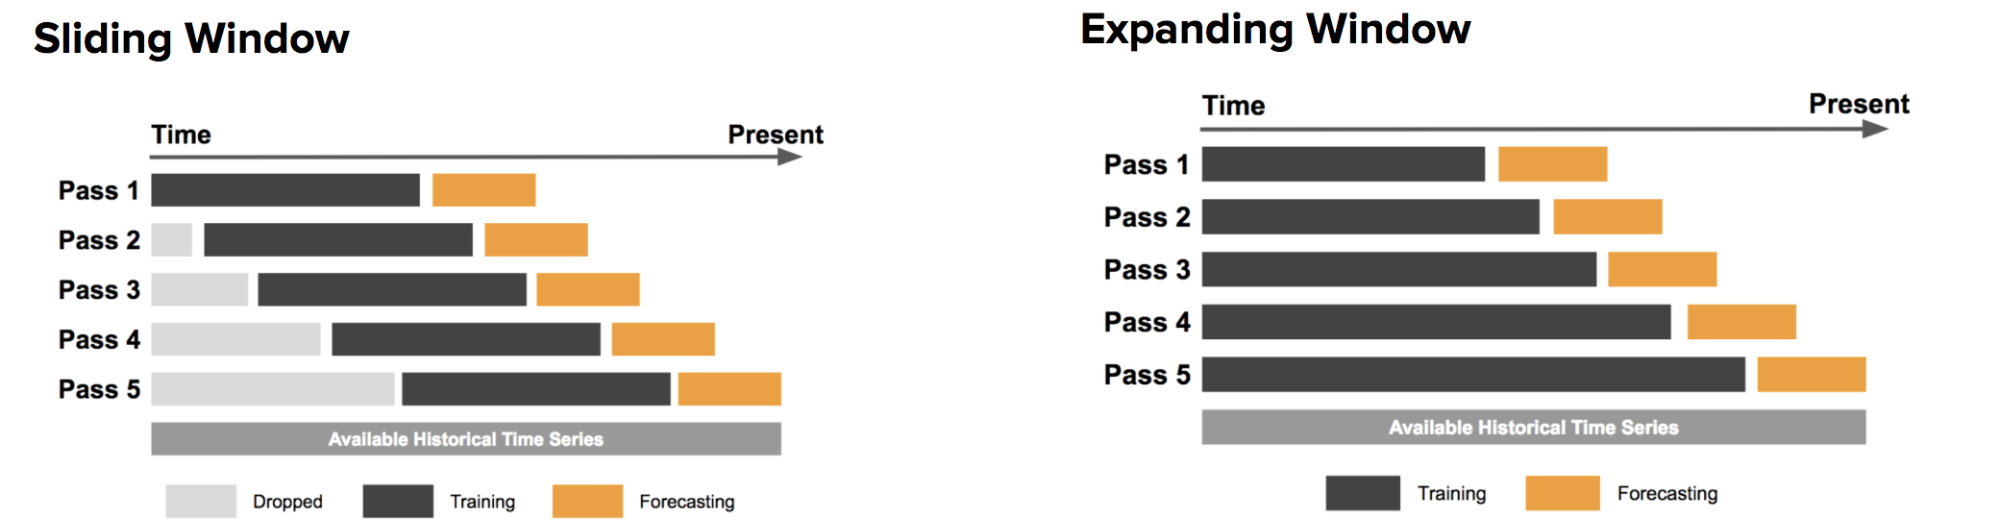
\includegraphics[scale=0.2]{images/methodology/sliding-expanding-windows}}
\end{figure}

Expanding windows are used in this project because they reuse more data, data is scarce specially in the monthly aggregation.
All the models are trained with this strategy, and their final performance is computed by averaging the performance in all the windows.
The model obtaining the lowest MAE will be the selected as best and used for forecasting.

Concretely, 6 windows will be used on this cross validation process, with a test partition of size the forecasting horizon, which changes depending on if we are forecasting in a hourly, daily or monthly basis.

\subsection{ML models data preprocessing}
In statistical time series models as ARIMA, data can be directly introduced in the model without restructuring it.
But when we use ML-based architectures, data has to be reshaped so the models can recover autocorrelation.
That is why the author arranges it in the tabular form described in Figure \ref{fig:ml-arrangement}.
On it, the response (price) and predictors (as could be demand or generation) are included together with some response lags.
In this way, the ML model is capable of capturing the autocorrelation.

\begin{figure}[H]
\centering
    \caption{Tabular form in which data is disposed for ML models. On it, n is the number of observations in the time series and k is the number of lags in use.}
    \label{fig:ml-arrangement}
    \fbox{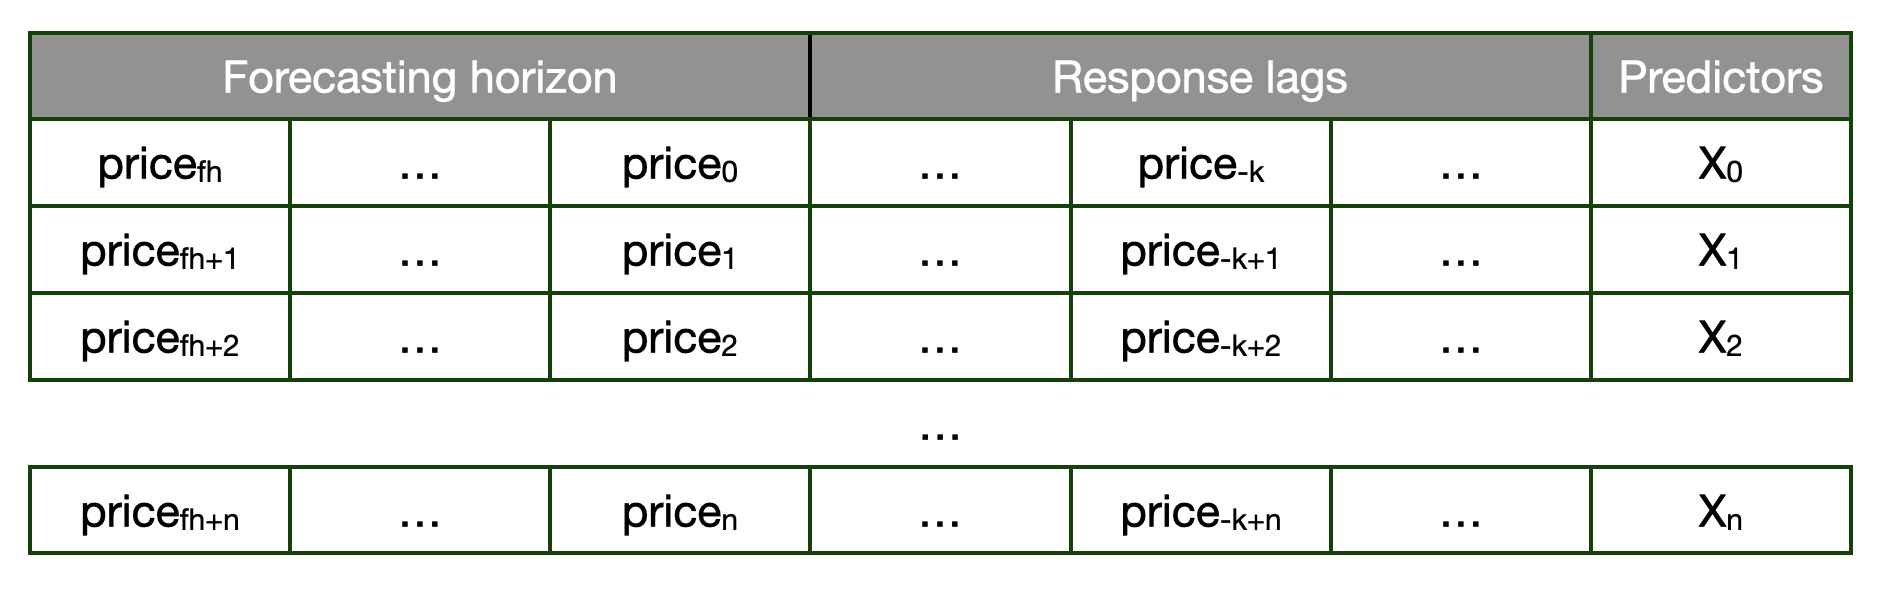
\includegraphics[scale=0.4]{images/methodology/ml_arrangement}}
\end{figure}

This preprocessing is automatically done by \textit{make\_reduction()} function.
On it, need to be specified the parameter \text{strategy}: there are two possible strategies to forecast each value in the forecasting horizon, direct and recursive.
The former creates one model for each value in the forecasting horizon, the latter applies a recursive process in which each new prediction is based on the previous one \cite{direct-recursive-forecasting}, so only one model is created. See Figure \ref{fig:direct-recursive-forecasting}. Recursive strategy is what is used on this project, as it is more efficient (although some performance is lost)

\begin{figure}[H]
\centering
    \begin{subfigure}{.45\textwidth}
        \centering
        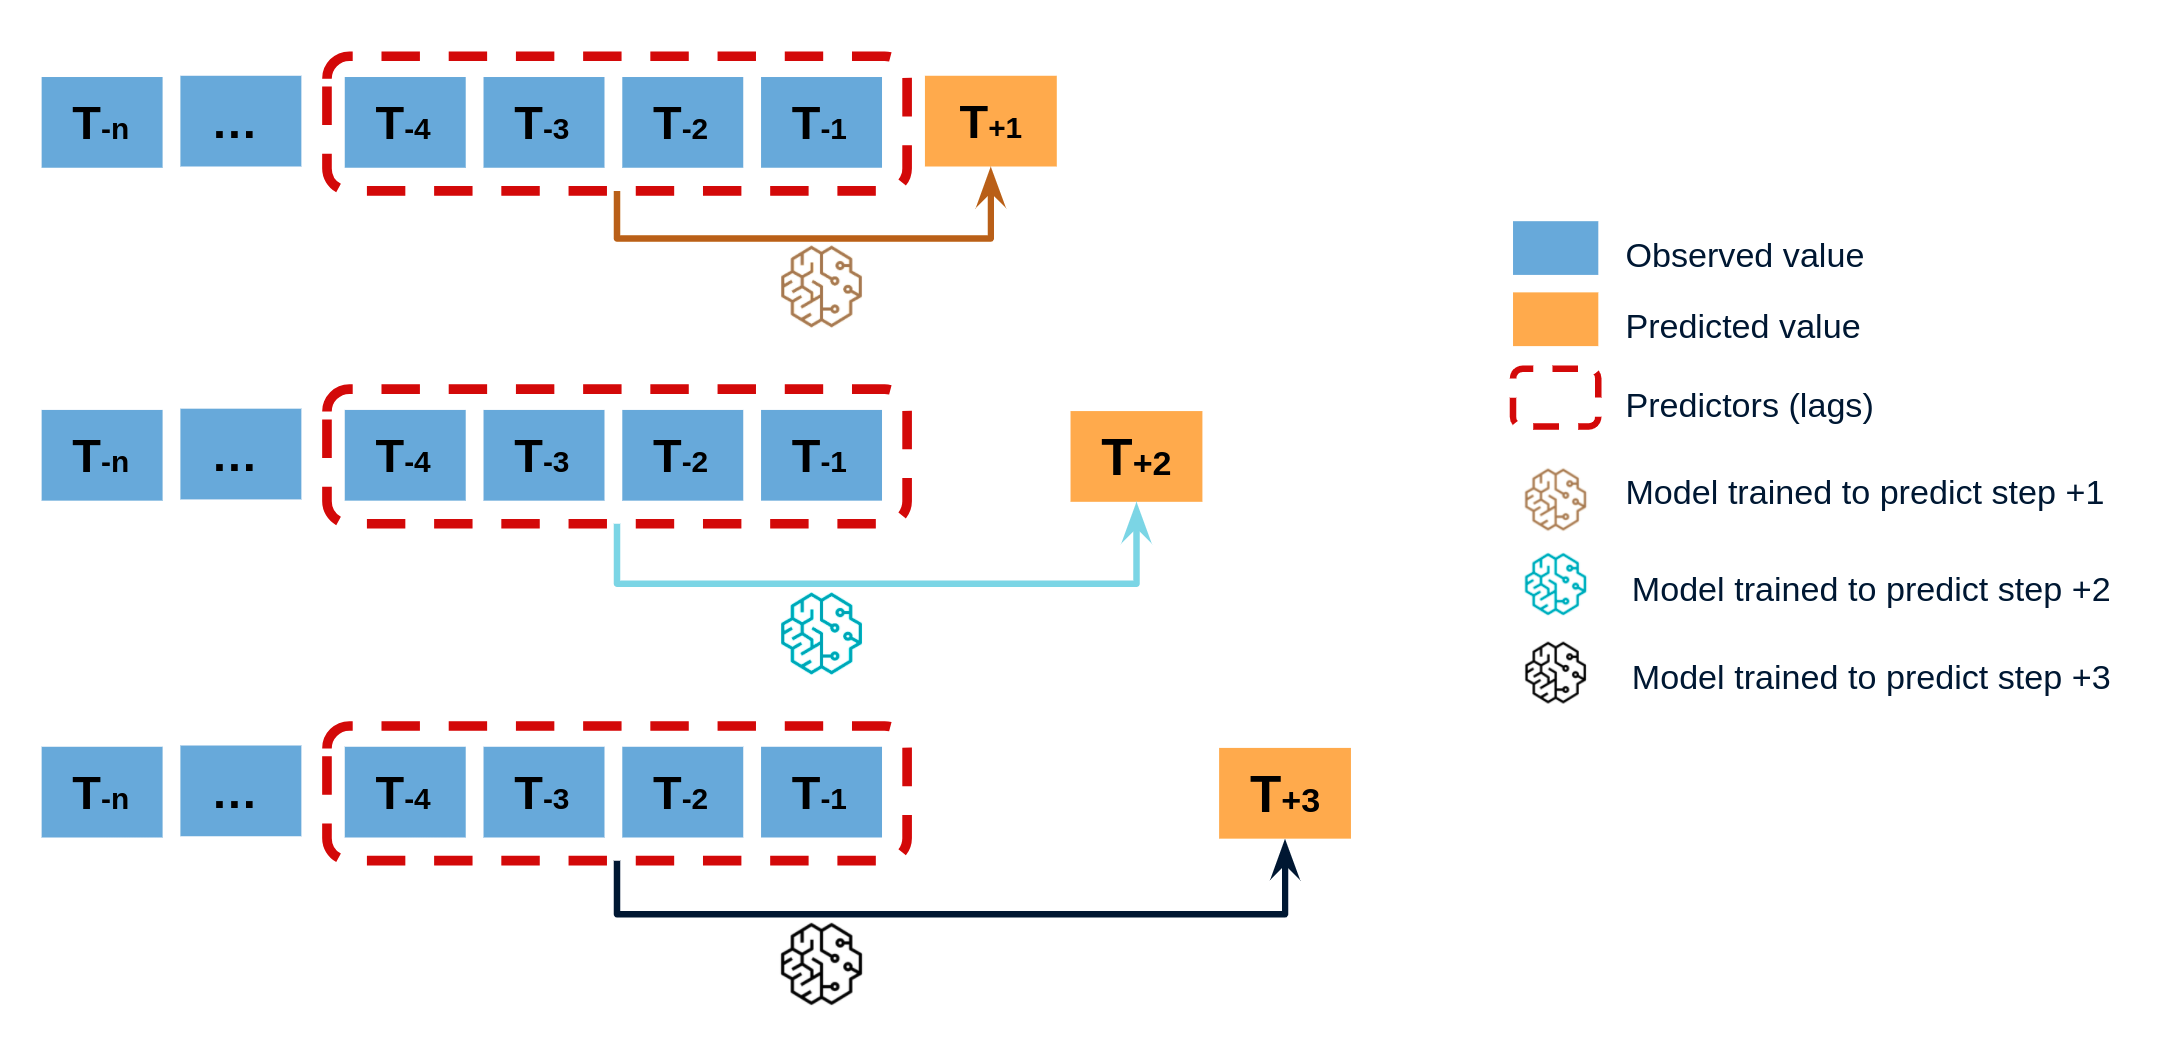
\includegraphics[width=1\linewidth]{images/methodology/direct-multi-step-forecasting}
        \caption{Direct forecasting.}
    \end{subfigure}
    \begin{subfigure}{.45\textwidth}
        \centering
        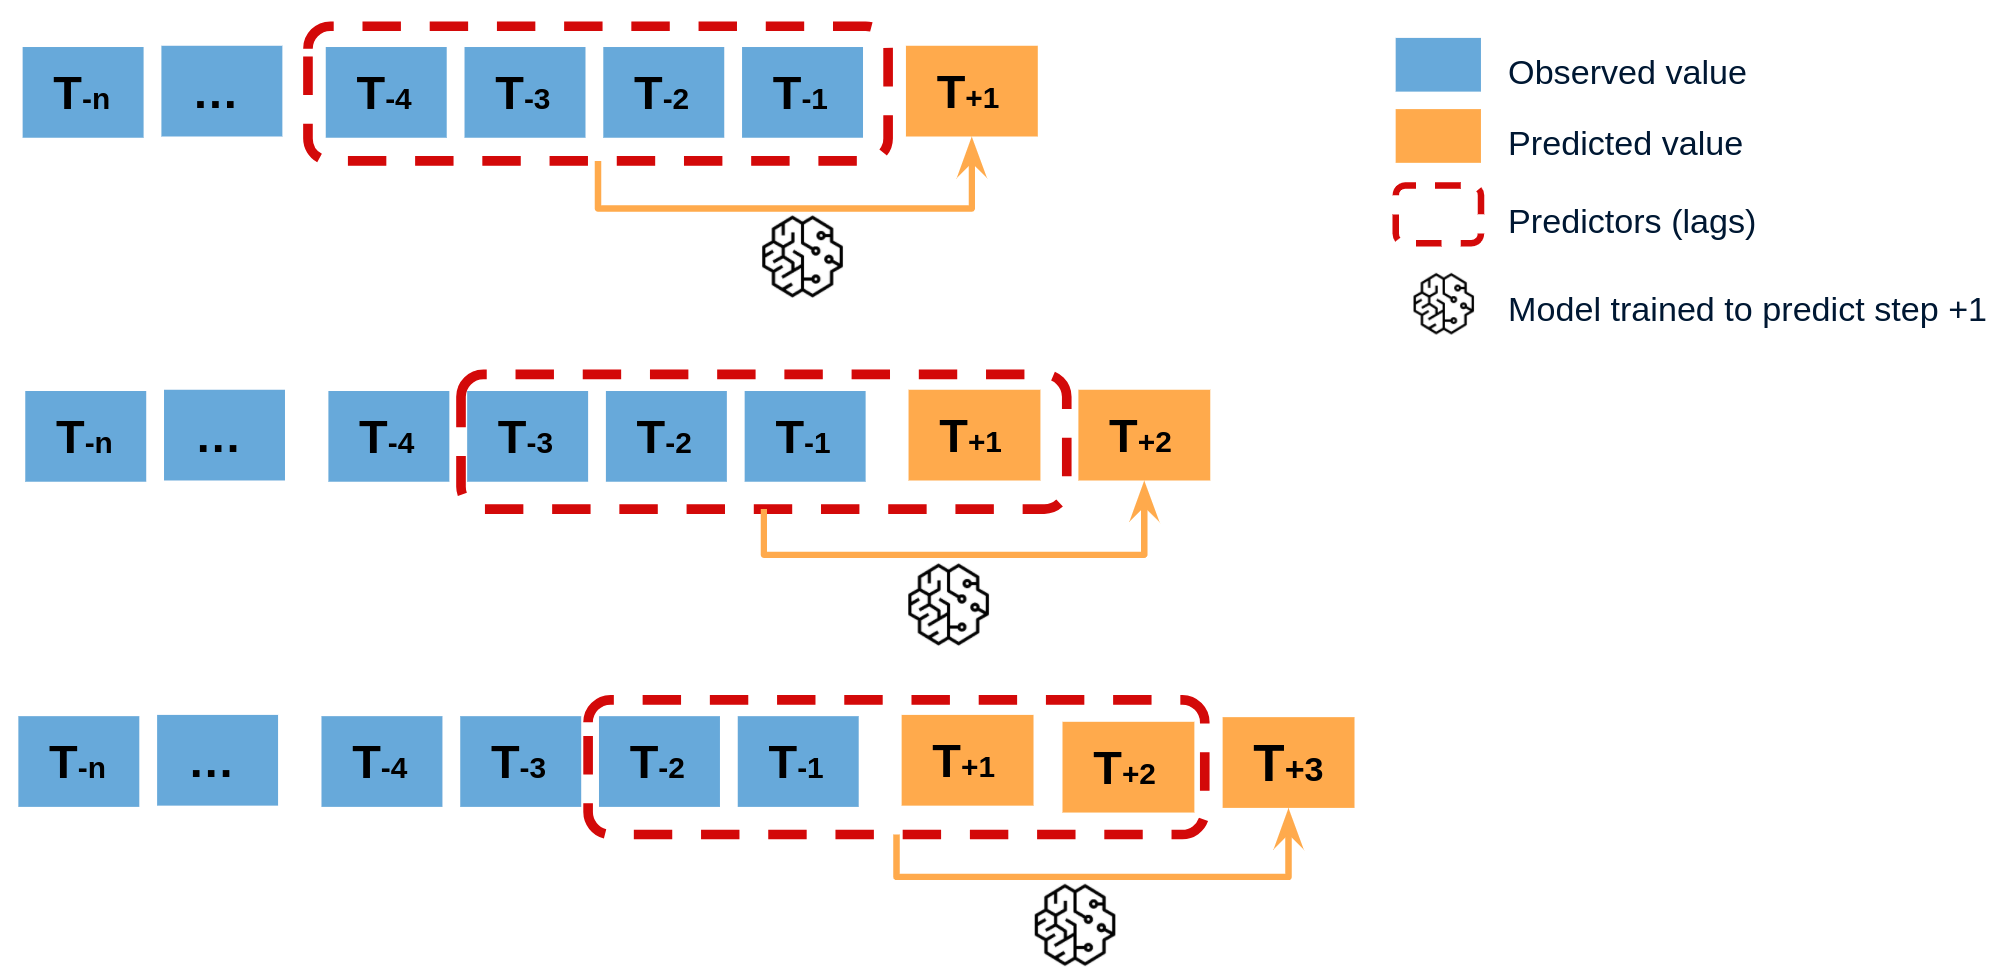
\includegraphics[width=1\linewidth]{images/methodology/recursive-mutistep-forecasting}
        \caption{Recursive forecasting.}
    \end{subfigure}

    \caption{Direct vs recursive forecasting strategies.}
    \label{fig:direct-recursive-forecasting}
\end{figure}

\section{Predictor's importance}

